\documentclass[12pt,t]{beamer}
\usepackage{pslatex}
\usetheme{Berkeley}
\useoutertheme{KUlogo}
\usecolortheme{KUhorse}
\title{Making Woody Parallel}
\subtitle{Applying Parallel Computing to decision trees}
% \author{}
\institute{Hugh McGrade \texttt{wbr412@alumni.ku.dk}\\%
  Mads Obitsø \texttt{scr411@alumni.ku.dk}\\%
  Titus Robroek \texttt{robroek@di.ku.dk}\\ - \\
  Department of Computer Science DIKU}
\date[]{\today}

\usepackage{listings}
\usepackage{wrapfig}
\usepackage{graphics}
\usepackage{color}
\definecolor{lightgray}{rgb}{.9,.9,.9}
\newsavebox\lstbox
\newsavebox\lstboxtwo
\newsavebox\lstboxthree
\newsavebox\lstboxfour
\newsavebox\lstboxfive

\usepackage{xcolor}
\usepackage{pgfplots}
\pgfplotsset{compat=1.15}
\definecolor{bblue}{HTML}{1010E0}
\definecolor{rred}{HTML}{D03030}
\definecolor{ggreen}{HTML}{40E040}
\definecolor{ppurple}{HTML}{800080}
\definecolor{yyellow}{HTML}{EECC20}
\definecolor{llightblue}{HTML}{6F91DD}

\usepackage{caption}
\usepackage{subcaption}

\lstset{basicstyle=\small}


\allowdisplaybreaks

\begin{document}

\frame[plain]{\titlepage}

\begin{frame}
  \frametitle{Introduction}
  %Content goes her

\section{Introduction}

\begin{itemize}
  \item What is Woody?
  \item Decision trees and Machine Learning
\end{itemize}
%
% Random forests have long been a staple of machine learning. They offer a fast, reliable way of tackling classification and regression problems. Their practical ability, however, is not without bounds. Scaling up trees to huge sizes, having massive numbers of trees and processing gigantic numbers of queries all show the limits of current processing technology. This report is about utilising GPU computing to scale up decision tree processing.
%
% In order to utilise GPU computing for decision tree processing we implemented the key part of random forest prediction - the evaluation of a single decision tree with test data - in Futhark. This implementation is intended for use as a replacement for the existing decision tree processing in the Woody random forest framework \cite{woody}.
%
% %motivation
% This research aims to investigate ways to scale the evaluation of large decision trees on large data. Larger decision trees may be very useful for some areas of research. The field of remote sensing, for example, requires the evaluation of decision trees on large and potentially complex datasets such as satelite images \cite{randomforest}. The speed improvements which could be achieved by parallelising this evaluation would make it possible to apply random forest models to larger problems.

\end{frame}
\begin{frame}
  \frametitle{Working with Woody}
  \framesubtitle{Decision tree evaluation}
\section{Working with Woody}

\subsection{Decision tree evaluation}

% The evaluation of a single decision tree in a random forest prediction takes a single decision tree from the forest and a matrix of test data. From this a vector of predictions is produced, each of which corresponds to the decision made from evaluating the decision tree for a given row of the test data. These rows can either be specified by an indices array mapping decision indices to row indices, or simply by taking each row in order.

\begin{wrapfigure}{R}{0.35\textwidth}
\centering
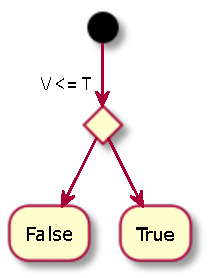
\includegraphics[width=0.35\textwidth]{decision_node}
% \caption{\label{fig:frog1}A non-leaf node within a tree. The query is directed based on one of it's data elements (V) tested against a specific threshold(T).}
\end{wrapfigure}
A decision tree consists of nodes.
Non-leaf nodes consist of a conditional check, where:
\begin{itemize}
\item V: Feature value checked for this node
\item T: Threshold value of the node that is checked against
\end{itemize}


% Each node of the decision tree specifies a threshold for proceeding on its left or right branch and the feature (column of the test data) which should be used to evaluate this threshold. In evaluation this continues until a leaf node is reached which is then the result.

\end{frame}

\begin{frame}
  \frametitle{Working with Woody}
  \framesubtitle{Extracting from Woody}
\subsection{Extracting from Woody}

\begin{enumerate}
  \item Python library run against a dataset
  \item Split data into training and test set
  \item Fit on training set to create a forest of trees
  \item Run predictions with test set on this forest
\end{enumerate}

\end{frame}


\begin{frame}
  \frametitle{Working with Woody}
  \framesubtitle{Interoperation of Woody and Futhark}
\subsection{Interoperation of Woody and Futhark}

\begin{figure}
\centering
\begin{subfigure}{.5\textwidth}
  \centering
  
\includegraphics[width=.5\linewidth]{opencl_logo}
  % \caption{A subfigure}
  \label{fig:pyopencl}
\end{subfigure}%
\begin{subfigure}{.5\textwidth}
  \centering
  
\includegraphics[width=.5\linewidth]{opencl}
  % \caption{A subfigure}
  \label{fig:opencl}
\end{subfigure}
% \caption{A figure with two subfigures}
\label{fig:test}
\end{figure}

Run as a library or run stand-alone?

% The Futhark compiler features code generation for the PyOpenCL library, allowing Futhark code compiled for OpenCL to be called from Python. This generated code accepts NumPy arrays as Futhark arrays. As Woody is written in Python, we are able to compile our Futhark library for PyOpenCL and use it as a library in Woody's Python code.

\end{frame}
\begin{frame}
  \frametitle{Working with Woody}
  \framesubtitle{Tree and test data encoding for Futhark}
\subsection{Tree and test data encoding for Futhark}

In order to pass the tree and test data from Woody to Futhark, we encoded each as a series of flat arrays.

\begin{itemize}
  \item \texttt{treeLeftid}
  \item \texttt{treeRightid}
  \item \texttt{treeFeature}
  \item \texttt{treeThres\_or\_leaf}
\end{itemize}

\begin{itemize}
  \item \texttt{Xtest}
  \item \texttt{nXtest}
  \item \texttt{dXtest}
\end{itemize}

%
% In the case of the tree, this took the form of four arrays giving the properties of each node by index: \texttt{treeLeftid}, \texttt{treeRightid}, \texttt{treeFeature} and \texttt{treeThres\_or\_leaf}. These give the left child ID, right child ID, feature index and threshold respectively.
%
% The test data matrix is described by a single array containing each of the test values (\texttt{Xtest}) and values \texttt{nXtest} and \texttt{dXtest} which give the shape of the matrix.

\end{frame}

\begin{frame}
  \frametitle{Writing Futhark}
  \framesubtitle{Basic Futhark implementation}
\section{Writing Futhark}
\subsection{Basic Futhark implementation}


\begin{figure}
\centering
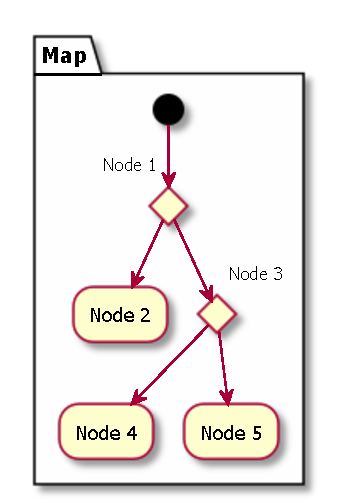
\includegraphics[width=0.4\textwidth]{tree_basic}
% \caption{\label{fig:frog2}Our basic futhark implementation. Every query is tested on a tree by mapping over all queries.}
\end{figure}

\end{frame}
\begin{frame}[fragile]
  \frametitle{Writing Futhark}
  \framesubtitle{Basic Futhark implementation}
  % \begin{lrbox}{\lstbox}
  \begin{minipage}{\textwidth}
  \begin{lstlisting}[language=Haskell, breaklines]
    unsafe map (\ i ->
    let idx = if dindices > 0 then indices[i] else i
    let row_start = idx * dXtest
    in loop node_id = TREE_ROOT_ID
          while treeLeftid[node_id] != TREE_CHILD_ID_NOT_SET do
                if Xtest[row_start + treeFeature[node_id]] <= treeThres_or_leaf[node_id]
                  then treeLeftid[node_id]
                  else treeRightid[node_id]
               ) (iota n_preds)
  \end{lstlisting}
  \end{minipage}
  % \end{lrbox}
%
% We started by producing a translation of Woody's single tree query into Futhark. Woody's version is parallelised using OpenMP over the trees in the forest. The Futhark for this is as follows:
%
% \vspace{1ex}
% \begin{lrbox}{\lstbox}
% \begin{minipage}{\textwidth}
% \begin{lstlisting}[language=Haskell, breaklines]
%   unsafe map (\ i ->
%   let idx = if dindices > 0 then indices[i] else i
%   let row_start = idx * dXtest
%   in loop node_id = TREE_ROOT_ID
%         while treeLeftid[node_id] != TREE_CHILD_ID_NOT_SET do
%               if Xtest[row_start + treeFeature[node_id]] <= treeThres_or_leaf[node_id]
%                 then treeLeftid[node_id]
%                 else treeRightid[node_id]
%              ) (iota n_preds)
% \end{lstlisting}
% \end{minipage}
% \end{lrbox}
% \vspace{1ex}
%
% \colorbox{lightgray}{\usebox\lstbox}
%
% This implementation parallelises the evaluation over the rows of the test data using a map over each prediction. The function to be mapped uses a Futhark while loop which assigns the root of the tree to \texttt{node\_id} and subsequently the result of the loop body which gives the next node. The loop terminates when a leaf node is reached and thus the function returns the ID of the leaf node.
%
% This is clearly not an idiomatic Futhark implementation and is included here only as a Futhark translation of the original C. The parellelisation approach is useful in that it distributes the trees, all of which have the same size.

\end{frame}
\begin{frame}
  \frametitle{Writing Futhark}
  \framesubtitle{Layered Futhark implementation}
\subsection{Layered Futhark implementation}

\begin{figure}
\centering
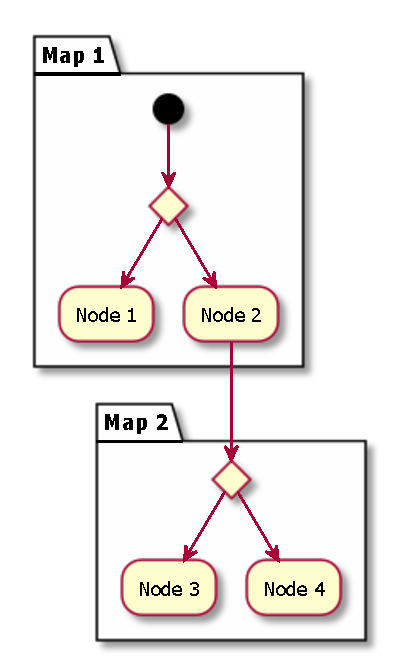
\includegraphics[width=0.4\textwidth]{tree_flat}
% \caption{\label{fig:frog3}Our layered Futhark implementation. Every layer of the tree is executed over the queries as a map, resulting in as many maps as there are layers in the tree.}
\end{figure}

\end{frame}
\begin{frame}[fragile]
  \frametitle{Writing Futhark}
  \framesubtitle{Layered Futhark implementation}
  \begin{minipage}{\textwidth}
  \begin{lstlisting}[language=Haskell, breaklines]
  loop node_array for row in iota(depth) do
      unsafe map (\ (node_id, data_row_start) ->
                   if (treeLeftid[node_id] != 0)
                      then (if Xtest[data_row_start + treeFeature[node_id]] <= treeThres_or_leaf[node_id]
                          then treeLeftid[node_id]
                          else treeRightid[node_id])
                      else node_id)
                      (zip node_array data_row_starts)
  \end{lstlisting}
  \end{minipage}
% A different approach to parallelising tree querying in Futhark is to combine the basic implementation's \texttt{map} and \texttt{while} loop into a single \texttt{map} and repeat this sequentially for each layer of the tree. This way we can remove the \texttt{while} loop out of the program.
%
% This is accomplished with an outer loop over every layer of the tree and an inner map over each node in the row. For the map, the nodes array (\texttt{node\_array}) and the data rows array (\texttt{data\_row\_starts}) are joined using a zip and mapped with a function producing the next node for each. This new array of node IDs is then used for the next iteration.
%
% \vspace{1ex}
% \begin{lrbox}{\lstboxtwo}
% \begin{minipage}{\textwidth}
% \begin{lstlisting}[language=Haskell, breaklines]
% loop node_array for row in iota(depth) do
%     unsafe map (\ (node_id, data_row_start) ->
%                  if (treeLeftid[node_id] != 0)
%                     then (if Xtest[data_row_start + treeFeature[node_id]] <= treeThres_or_leaf[node_id]
%                         then treeLeftid[node_id]
%                         else treeRightid[node_id])
%                     else node_id)
%                     (zip node_array data_row_starts)
% \end{lstlisting}
% \end{minipage}
% \end{lrbox}
% \vspace{1ex}
%
% \colorbox{lightgray}{\usebox\lstboxtwo}

\end{frame}
\begin{frame}
  \frametitle{Writing Futhark}
  \framesubtitle{Filtering Futhark implementation}
\subsection{Filtering Futhark implementation}

\begin{itemize}
  \item Layered provides a structured way of iterating over layers
  \item Many passes end early
  \item These are still considered by the maps
\end{itemize}

% Our layered Futhark implementation applies a map for every layer of the tree. Some queries, however, will have hit a leaf at some point. The current implementation, however, still attempts to apply a map for every query, even if it has stopped at a leaf. Our next implementation attempts to solve this issue.
% We want to avoid repeatedly processing those paths which have reached a leaf node. We do this by applying a filter operation on our iterations. We filter the queries based on them have reached a leaf node or not. This causes the map to only be applied to "live" paths.
%
% Following the tree traversal a sort is applied based on the test data rows to produce a prediction for each row.
%
% \vspace{1ex}
% \begin{lrbox}{\lstboxthree}
% \begin{minipage}{\textwidth}
% \begin{lstlisting}[language=Haskell, breaklines]
%   let nodes = zip node_array data_row_starts
%   let leaves = []
%   let (_, leaves) = loop (nodes, leaves) for row in iota(depth) do
%                     let new_nodes = (unsafe map next_node nodes)
%                     in (unsafe filter is_not_leaf new_nodes,
%                         leaves ++ (unsafe filter is_leaf new_nodes))
%   let result = map (\ (a, _) -> a)
%                     (radix_sort_by_key (\ (_, a) -> a)
%                                         i32.num_bits
%                                         i32.get_bit
%                                         leaves)
%   in result
% \end{lstlisting}
% \end{minipage}
% \end{lrbox}
% \vspace{1ex}
%
% \colorbox{lightgray}{\usebox\lstboxthree}
%
% This implementation again parallelises the queries by applying a map to each row. As it prunes the tree we can expect it to perform better on larger, deeper and less balanced trees.

\end{frame}
\begin{frame}
  \frametitle{Writing Futhark}
  \framesubtitle{Treesolver Precompute}
\subsection{Treesolver Precompute}

\begin{figure}
\centering
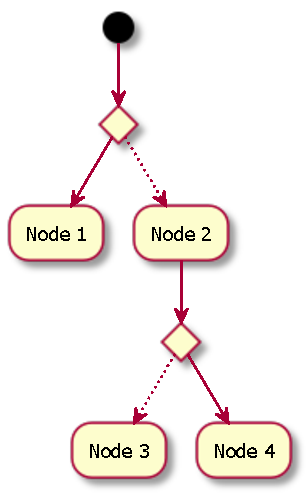
\includegraphics[width=0.4\textwidth]{tree_traverse}
% \caption{\label{fig:frog3}A visualisation of a traverse tree/matrix. Node 0 points to node 1 and node 2 points to node 4 for this specific query. Walking through the tree will thus result in this query be classified as node 1.}
\end{figure}

\end{frame}
\begin{frame}[fragile]
  \frametitle{Writing Futhark}
  \framesubtitle{Treesolver Precompute}
  \begin{minipage}{\textwidth}
  \begin{lstlisting}[language=Haskell, breaklines]
  let next_node
    (row: []f64)
    ((left, right, feature, thres) : (i32, i32, i32, f64)) : i32 =
    if row[feature] <= thres then left else right

  let make_next_tree
     (tree: [](i32, i32, i32, f64))
     (row : []f64) : []i32 =
     map (next_node row) tree

  let traverse
     (next_nodes: []i32): i32 =
     let (last, current) = (0, next_nodes[0])
     let (result, _) = loop (last, current) while current != 0 do (current, next_nodes[current])
     in result

  let nodes = zip4 treeLeftid treeRightid treeFeature treeThres_or_leaf
  let rows = unflatten nXtest dXtest Xtest

  let next_nodes = unsafe map (make_next_tree nodes) rows

  in unsafe map traverse next_nodes

  \end{lstlisting}
  \end{minipage}
%
% A further approach we took to implement decision tree querying in Futhark was to compute the outcome of each tree node prior to traversing the tree. This greatly increases the scope for parallelism in the evaluation of tree thresholds as every node can now be computed independently. To do this we map the function \texttt{make\_next\_tree} (with the tree) to every row of the data. This further maps the function \texttt{next\_node} (with the row of the data) to every node of the tree, creating a direction matrix which for each node (by index) gives the following node's index. This is shown in figure 4. The tree is then trivially traversed by following these pointers from the root node.
%
% \vspace{1ex}
% \begin{lrbox}{\lstboxfour}
% \begin{minipage}{\textwidth}
% \begin{lstlisting}[language=Haskell, breaklines]
% let next_node
%   (row: []f64)
%   ((left, right, feature, thres) : (i32, i32, i32, f64)) : i32 =
%   if row[feature] <= thres then left else right
%
% let make_next_tree
%    (tree: [](i32, i32, i32, f64))
%    (row : []f64) : []i32 =
%    map (next_node row) tree
%
% let traverse
%    (next_nodes: []i32): i32 =
%    let (last, current) = (0, next_nodes[0])
%    let (result, _) = loop (last, current) while current != 0 do (current, next_nodes[current])
%    in result
%
% let nodes = zip4 treeLeftid treeRightid treeFeature treeThres_or_leaf
% let rows = unflatten nXtest dXtest Xtest
%
% let next_nodes = unsafe map (make_next_tree nodes) rows
%
% in unsafe map traverse next_nodes
%
% \end{lstlisting}
% \end{minipage}
% \end{lrbox}
% \vspace{1ex}
%
% \colorbox{lightgray}{\usebox\lstboxfour}
%
% We found this approach was far better suited to using an idiomatic Futhark style and made the potential for parallelisation clearer by separating tree travsersal. Future work could consider better flattening this approach.

\end{frame}
\begin{frame}[fragile]
  \frametitle{Writing Futhark}
  \framesubtitle{Treesolve Matrix}
\subsection{Treesolve Matrix}
\begin{minipage}{\textwidth}
\begin{lstlisting}[language=Haskell, breaklines]
let repeated_criteria = flatten (replicate nXtest treeFeature)
  let repeated_offsets = flatten (map (\ i -> replicate treelength i) (steps 0 nXtest dXtest))
  let flcr = map2 (+) repeated_offsets repeated_criteria
  let scattered_features = unsafe map (\ i -> Xtest[i]) flcr
  let threshold_result = map2 (<=) scattered_features (flatten (replicate nXtest treeThres_or_leaf))
  let left_or_right = (\ b l r -> if b then l else r)
  let repeatedLeft = flatten (replicate nXtest treeLeftid)
  let repeatedRight = flatten (replicate nXtest treeRightid)
  let directions = map3 left_or_right threshold_result repeatedLeft repeatedRight

  in unsafe map traverse (unflatten nXtest treelength directions)
\end{lstlisting}
\end{minipage}

% A similar approach is to again parallelise by mapping over all possible nodes and their corresponding data using a series of maps. This produces a series of matrices representing properties of the tree and results in the matrix \texttt{direction} which gives the following node from each node. As in the previous implementation, this is then trivially traversed to obtain the result.
%
% \vspace{1ex}
% \begin{lrbox}{\lstboxfive}
% \begin{minipage}{\textwidth}
% \begin{lstlisting}[language=Haskell, breaklines]
% let repeated_criteria = flatten (replicate nXtest treeFeature)
%   let repeated_offsets = flatten (map (\ i -> replicate treelength i) (steps 0 nXtest dXtest))
%   let flcr = map2 (+) repeated_offsets repeated_criteria
%   let scattered_features = unsafe map (\ i -> Xtest[i]) flcr
%   let threshold_result = map2 (<=) scattered_features (flatten (replicate nXtest treeThres_or_leaf))
%   let left_or_right = (\ b l r -> if b then l else r)
%   let repeatedLeft = flatten (replicate nXtest treeLeftid)
%   let repeatedRight = flatten (replicate nXtest treeRightid)
%   let directions = map3 left_or_right threshold_result repeatedLeft repeatedRight
%
%   in unsafe map traverse (unflatten nXtest treelength directions)
% \end{lstlisting}
% \end{minipage}
% \end{lrbox}
% \vspace{1ex}

\colorbox{lightgray}{\usebox\lstboxfive}

\end{frame}
\begin{frame}
  \frametitle{Experiment}
  \framesubtitle{Experimental Setup}
\section{Experiment}
\subsection{Experimental Setup}

To evaluate our Futhark implementation, we performed various comparisons with the woody implementation.

--Perhaps add an extra slide with an overview of the framework as an image?
Itemize the tests--

% To evaluate our Futhark implementation, we performed various comparisons with the woody implementation of \verb!cpu_query_tree!.
%
% All experiments were performed on a GPU node with two Intel(R) Xeon(R) CPU E5-2650 v2 processors at 2.60GHz (32 cores, 2 threads per core) and two GeForce GTX 780 Ti graphics cards.
%
% We wanted to both compare our predictions from Futhark to those from Woody and to measure and compare the runtimes with varying tree sizes and amount of predictions.
% To accomplish this, we modified parts of the Woody codebase and wrote a set of python scripts\footnote{The scripts can be run to recreate our comparisons and measuring. They can be found here: https://github.com/HughMcGrade/woody/tree/master/experiments/parallel. Run \texttt{python launch.py} from the directory \texttt{experiments/parallel}}. that orchestrates the testing and measuring.
% The scripts will generate and fit a forest based on the given training size and optional testing size, where testing size determines the number of predictions to be made. It will then do a large number of predictions with the first tree of the forest, using in turn woody and all of our Futhark programs. After measuring running times, all predictions from Futhark programs are compared to those from Woody.
%
%
% We measure the runtime of the Woody implementation directly in Python. The runtimes of the Futhark programs are measured using the \verb!-t! argument to Futhark programs. This might give an unfair overhead to the woody implementation and make the result skewed towards the Futhark implementations. We call Futhark from Python through \verb!os.system()! instead of compiling our Futhark programs to Python modules and calling them directly from Python. Using modules might give a more practical measurement for comparisons.
%
% All programs are run 10 times and the average of those runtimes is used for the comparisons. The dataset used is the covtype dataset, already available in woody.

\end{frame}
\begin{frame}
  \frametitle{Experiment}
  \framesubtitle{Results: Varying train data size}
\subsection{Results}
% We have included two different comparisons. Both figures show runtime comparisons of predictions on single tree, between the Woody implementation and our 5 Futhark implementations. Two of the programs, matrix and prune in the plots, fail with larger data but are included where they do run.
%
% Figure \ref{plot:runtime1} shows runtime comparisons for varying tree sizes. The training size affects the size of the tree, with small training sizes giving very small trees. All measurements in \ref{plot:runtime1} were made with 116203 predictions, the size of the standard test set.
%
%
% Figure \ref{plot:runtime2} shows runtime comparisons for increasing amounts of predictions. The number of queries is set equal to the training size.


\begin{figure}[h]
  \centering
  \begin{tikzpicture}[thick,scale=0.7, every node/.style={scale=0.7}]
  \begin{axis}[
    title={Microseconds used predicting a single tree as average of 10 runs},
    title style = {xshift=-2cm, font=\bfseries},
    width  = \textwidth,
    height = 8cm,
    major x tick style = transparent,
    ybar=2*\pgflinewidth,
    bar width=5pt,
    ymajorgrids = true,
    ylabel = {Microseconds},
    symbolic x coords={1000, 10000, 100000, 200000, 300000, 400000},
    xtick = data,
    xlabel = {Train data size},
    scaled y ticks = false,
    enlarge x limits=0.10,
    ymin=0,
    legend columns=3,
    legend cell align=left,
    legend pos =outer north,
    legend style={
      at={(0.5,1.35)},
      anchor=north,
      column sep=1ex
    }
    ]
% cpu predict
    \addplot[style={bblue,fill=bblue,mark=none}]
    coordinates {
      (1000,   24751)
      (10000,  27794)
      (100000, 30553)
      (200000, 29728)
      (300000, 33381)
      (400000, 34311)
    };
% treesolve basic
    \addplot[style={rred,fill=rred,mark=none}]
    coordinates {
      (1000,   532 )
      (10000,  781 )
      (100000, 934 )
      (200000, 1038)
      (300000, 1308)
      (400000, 1386)
    };
    % treesolve layer
    \addplot[style={yyellow,fill=yyellow,mark=none}]
    coordinates {
      (1000,   738)
      (10000,  1171)
      (100000,  1430)
      (200000,  1717)
      (300000, 1983)
      (400000, 1993)
    };
% treesolve filter
    \addplot[style={llightblue,fill=llightblue,mark=none}]
    coordinates {
      (1000,   9925 )
      (10000,  12096 )
      (100000, 16039 )
      (200000, 16886)
      (300000, 18021)
      (400000, 17960)
    };
% treesolve precompute
    \addplot[style={ggreen,fill=ggreen,mark=none}]
    coordinates {
      (1000,   6923)
      (10000,  0)
      (100000, 0)
      (200000, 0)
      (300000, 0)
      (400000, 0)
    };
% treesolve matrix
\addplot[style={ppurple,fill=ppurple,mark=none}]
coordinates {
  (1000,   6924)
  (10000,  0)
  (100000, 0)
  (200000, 0)
  (300000, 0)
  (400000, 0)
};
    \legend{cpu predict, treesolve basic, treesolve layer, treesolve filter, treesolve precompute, treesolve matrix}
  \end{axis}
\end{tikzpicture}

  % \caption{Measuring time to make 116203 predictions with increasing tree sizes. Two of the programs, precompute and matrix in the plots, fail with larger data but are included where they do run.}
  \label{plot:runtime1}
\end{figure}

\end{frame}
\begin{frame}
  \frametitle{Experiment}
  \framesubtitle{Results: Varying number of predictions}
\begin{figure}[h]
  \centering
  \begin{tikzpicture}[thick,scale=0.7, every node/.style={scale=0.7}]
  \begin{axis}[
    title={Microseconds used predicting a single tree as average of 10 runs},
    title style = {xshift=-2cm, font=\bfseries},
    width  = \textwidth,
    height = 8cm,
    major x tick style = transparent,
    ybar=2*\pgflinewidth,
    bar width=5pt,
    ymajorgrids = true,
    ylabel = {Microseconds},
    symbolic x coords={1000, 10000, 100000, 200000, 300000, 400000},
    xtick = data,
    xlabel = {Number of predictions made},
    scaled y ticks = false,
    enlarge x limits=0.10,
    ymin=0,
    legend columns=3,
    legend cell align=left,
    legend pos = outer north,
    legend style={
      at={(0.5,1.35)},
      anchor=north,
      column sep=1ex
    }
    ]
% cpu predict
    \addplot[style={bblue,fill=bblue,mark=none}]
    coordinates {
      (1000,   137)
      (10000,  1384)
      (100000, 25908)
      (200000, 54335)
      (300000, 89560)
      (400000, 121094)
    };

% treesolve basic
    \addplot[style={rred,fill=rred,mark=none}]
    coordinates {
      (1000,   64 )
      (10000,  108 )
      (100000, 862 )
      (200000, 1786)
      (300000, 3273)
      (400000, 4616)
    };

% treesolve flat
    \addplot[style={yyellow,fill=yyellow,mark=none}]
    coordinates {
      (1000,   253)
      (10000,  367)
      (100000,  1285)
      (200000,  2769)
      (300000, 4460)
      (400000, 5760)
    };
        % treesolve (what to call this one?)
    \addplot[style={llightblue,fill=llightblue,mark=none}]
    coordinates {
      (1000,   5743 )
      (10000,  8174 )
      (100000, 15240 )
      (200000, 28212)
      (300000, 33916)
      (400000, 37009)
    };
    % treesolve precompute
    \addplot[style={ggreen,fill=ggreen,mark=none}]
    coordinates {
      (1000,   93)
      (10000,  4683)
      (100000, 0)
      (200000, 0)
      (300000, 0)
      (400000, 0)
    };
% treesolve superflat
    \addplot[style={ppurple,fill=ppurple,mark=none}]
    coordinates {
      (1000,   95)
      (10000,  4682)
      (100000, 0)
      (200000, 0)
      (300000, 0)
      (400000, 0)
    };

    \legend{cpu predict, treesolve basic, treesolve layer, treesolve filter, treesolve precompute, treesolve matrix}
  \end{axis}
\end{tikzpicture}

  % \caption{Measuring time to make increasing amounts of predictions with increasing tree sizes. Two of the programs, precompute and matrix in the plots, fail with larger data but are included where they do run.}
  \label{plot:runtime2}
\end{figure}

\end{frame}
\begin{frame}
  \frametitle{Experiment}
  \framesubtitle{Evaluation}
\subsection{Evaluation}

\begin{itemize}
  \item Basic and layer are fast.
  \item GPU code scales better with bigger tests
\end{itemize}

\end{frame}
\begin{frame}
  \frametitle{Experiment}
  \framesubtitle{Future Research}
\subsection{Future Research}

\begin{itemize}
  \item Matrix and Precompute might be promising
  \item GPU code scales better with bigger tests
\end{itemize}



% The comparison shown in \ref{plot:runtime1} gives the runtimes for each of our five Futhark implementations and Woody's C implementation when varying the size of the training data producing the decision trees. Due to memory issues, the matrix and precompute implementations fail on larger data. These results show that the basic and layer implementations give substantial improvements in performance over Woody. The runtime of all programs grow slowly as the size of the training date increases.
%
% The comparison shown in \ref{plot:runtime2} gives the runtimes for each of our five Futhark implementations and Woody's C implementation when varying the number of predictions being made. These results show that the number of predictions has a far greater impact on the Woody implementation than on the Futhark implementation. The increase in Woody's runtime from 10.000 to 100.000 is quite large, where Futhark has only a marginal increase. Futhark seems to handle large tree sizes much faster than woody.
%
% In the future, it may be interesting to future investigate these parallel implementations. For example, more sophisticated techniques may be able to further improve the performance of the algorithms. Furthermore, it may be possible to streamline the precompute and matrix implementation.


\end{frame}
\begin{frame}
  \frametitle{Conclusion}
\section{Conclusion}

We have proposed a number of approaches to parallelising the evaluation of decision trees using Futhark. Our findings show that as a whole this parallelisation is promising for the performance of decision tree evaluation on large datasets.

\end{frame}

\begin{thebibliography}{}

\bibitem{randomforest}
Belgiu, Mariana, and Lucian Drăguţ. "Random forest in remote sensing: A review of applications and future directions." ISPRS Journal of Photogrammetry and Remote Sensing 114 (2016): 24-31.

\bibitem{woody}
Gieseke, Fabian, and Christian Igel. "Training Big Random Forests with Little Resources." arXiv preprint arXiv:1802.06394 (2018).

\end{thebibliography}


\end{document}
